% !TeX root = ../main.tex
% Add the above to each chapter to make compiling the PDF easier in some editors.

\chapter{Results}\label{chapter:results}

As explained in the previous chapter, this thesis follows several topic modeling approaches to 
obtain the most representative result that can be analyzed. To emphasize the approaches again, 
the first approach follows Martin's general recommendations and does not change any arguments. 
This BERTopic approach delivers around 7500 topics, which is too much to analyze and make sense 
of the results. 

The main reason behind the mass number of topics is \texttt{min\_cluster\_size} remaining at 20, 
allowing around five thousand topics with less than five thousand tweets. The other main reason 
is the diversity of the analyzed data. To determine the topics, sample data of 1\% of all collected 
tweets is used from a dataset that contains more than 200,000 daily tweets. 
When manually looking at the data, one can realize that even though the size is small, the topic 
can be related to a real-life event. Nevertheless, on the other hand, most of the topics can be 
combined or be in the outlier category.

With the experiences from the first approach, the second approach tries to minimize the 
cluster size of the topics to obtain a better result. When the \texttt{min\_cluster\_size} remained 
at 100, around 1000 topics were returned from the topic model. Similar to the first approach, 
this approach also covered the most significant topics. Because the cluster sizes are bigger 
with this approach, the topics are more challenging to label and categorize in one area. Although 
one can realize the similarities between these approaches in the top eight representative words, 
the representative tweets differ. These representative tweets are used in OpenAI prompt to label 
the topics, so the quality of these tweets is of high importance. In this approach, most 
representative tweets include three similar long texts with a high proportion of hashtags and 
mentions. That is also why almost half of the top 20 topics are demands or requests from the 
government, where many users and bots spam almost similar tweets to put the topic in trends, 
promoting politicians, parties, and specific agendas \parencite{secim2023}.
% add additional information here about bots and etc 

After considering these arguments, this thesis mainly analyzes the results of the first approach, 
where one can realize topic trends consisting of specific topics that make comparing and analyzing 
the results considerably more straightforward.

It is essential to mention that outliers are not mentioned via graphs but are remembered 
during the results. Although some approaches in this tried to redistribute outliers, outliers 
exist for a reason. As Grootendorst notes, outliers are to be expected, and pushing the 
output to have no outliers may not correctly represent the data. 

One disadvantage of following the default pipeline of BERTopic is that when the model is first trained, 
the biggest cluster is usually the outliers. However, when training the model and transforming 
the rest of the data, the outlier cluster is considered a usual topic cluster like any other. 
For instance, during one of the approaches, the model had more tweets in the outlier cluster 
while training than after transforming all the collected data, which might, on the one hand, 
cause lots of meaningless topics and, on the other hand, not accurately represent the data. 
There are several new approaches that BERTopic supports that overcome that issue. 
One can try \textit{Online Topic Modeling} to incrementally train the model, or 
\textit{Merge Multiple Fitted Models} approach, where multiple models are trained and, in the end, 
merged so that no information is lost. These approaches are discussed in~\autoref{section:future_work}.

\begin{table}[htb] % second approach without outleirs
    \centering
    \small
    \begin{tabular}{|>{\hspace{0pt}}m{0.35\linewidth}|>{\hspace{0pt}}m{0.55\linewidth}|} 
    \hline
    \normalsize{\textbf{Topic Label}}                                 & \normalsize{\textbf{Representative Words}}                                                                                                                \\ 
    \hline\hline
    Political Discussions	& \footnotesize{aysedogan1955, yirmiucderece, hassa61, furkancerkes, secimtr2023, cenginyurt52, aykiricomtr, pusholder} \\
    Opposition Candidates 	& \footnotesize{oy, kılıçdaroğlu, oyları, seçmeni, oylar, vermem, aday, seçimde} \\
    Erdogan \& Nationalism 	& \footnotesize{türk, turkey, türkiye, yüzyılı, türkiyeyüzyılı, stanbul, milliyetçisi, cumhuriyeti} \\
    Religious Wishes	& \footnotesize{allah, versin, eylesin, müslüman, razı, mekanı, namaz, dini} \\
    Political Discussions \& Criticisms	& \footnotesize{cır, terketmek, denilince, uyruklu, ayrilmis, muharremin, vezir\_yuce, bahtiyar\_ergn} \\
    Criticism of Political Figures 	& \footnotesize{siyaset, siyasetin, siyasetiniz, siyasetçi, siyaseti, batsın, siyasete, siyasette} \\
    Opposition Coalition \& Criticism	& \footnotesize{erbakancayazan, örneğinde, yolunuzdan, iddialar, atıldılar, seçicez, ihtimalde, omurgasızlıktır} \\
    Treason Accusations	& \footnotesize{ülkeyi, ülkeye, ülke, ülkenin, ülkede, yağdanlıkları, unutturacaksınız, sığınmayın} \\
    Opposition Figures \& Preferences  & \footnotesize{oy, kılıçdaroğlu, oyları, seçmeni, oylar, vermem, aday, seçimde} \\
    Retirement System	& \footnotesize{emeklilik, kısmi, kademeli, emekli, emeklilikte, prim, 5000} \\
    Earthquake \& Demands	& \footnotesize{neticesiz, uzunca, deprem, depremin, süredir, atanma, yumuşak, depremde} \\
    Provocation \& Discussions	& \footnotesize{kızmaz, ahhh, vura, yanarız, soğancı, mitink, arsibjk1903bjk, baskan} \\
    Praise of Political Figures	& \footnotesize{başkanım, başkan, başbakan, başkanın, cumhurbaşkanım, selo, mehmetfatihser5, mehmetersoy57} \\
    Teachers \& Demands	& \footnotesize{öğretmen, öğretmenler, ataması, ilave, ücretli, öğretmenlere, cumhuriyetimizin, öğretmenlerin} \\
    Erdogan's Election Chance	& \footnotesize{rdoğana, erdoğan, erdoğanı, egemenlere, turda, tura, vereceğim, oyumu} \\
    \hline
    \end{tabular}
    \caption[Result of the topic modeling with labels and representative words.]
    {Result of the topic modeling with outlier redistribution. The top eight representative words
    from MMR model for each of the top 15 topics with their respective topic label 
    translated into English.}\label{tab:topic_modeling_results_1}
\end{table}

Right now I am testing.

\section{Analysis of data findings}

\begin{figure}[htb]
    \centering
    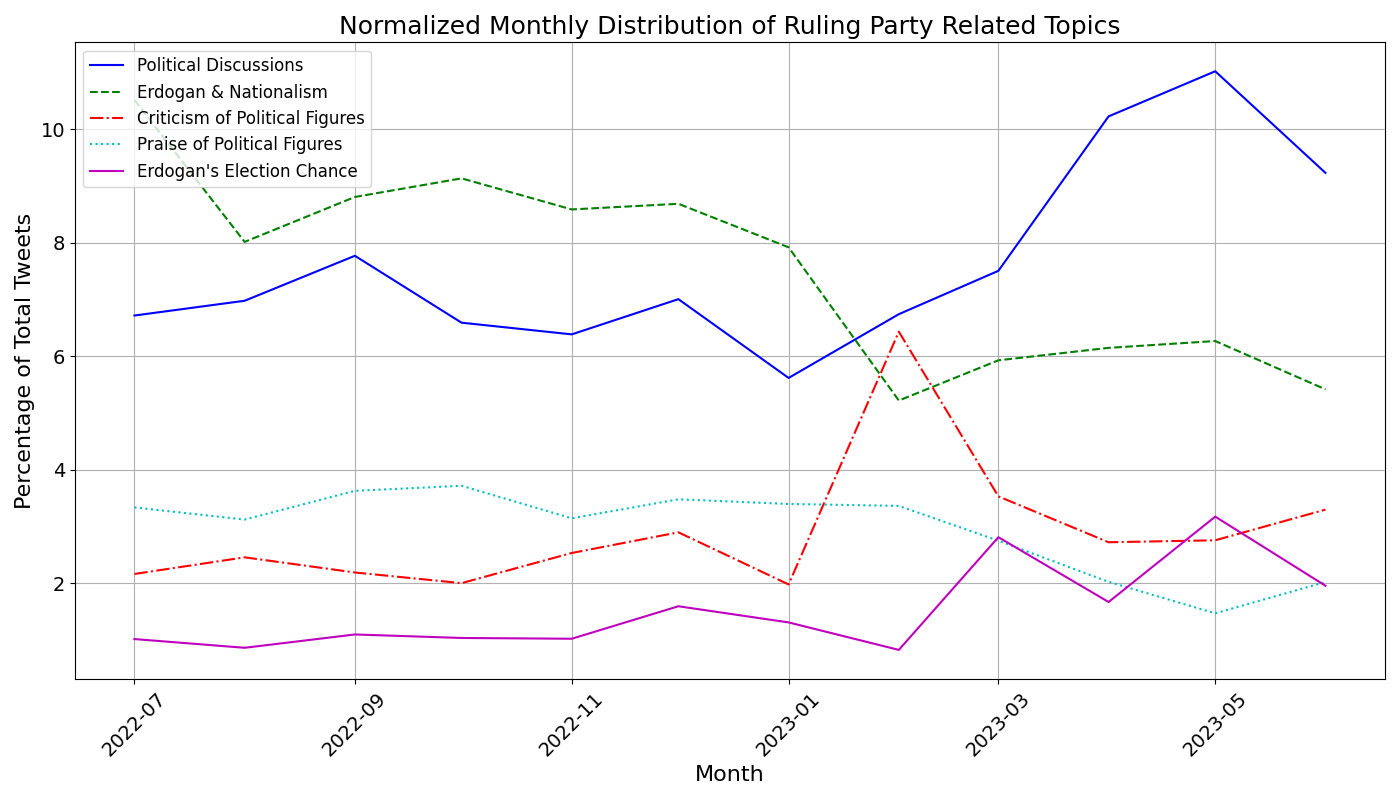
\includegraphics[width=\linewidth]{figures/normalized_akp_selected_topics_distribution_with_styles.png}
    \caption[Normalized monthly distribution of ruling party related topics]
    {Percentage of ruling party related topics in the top 50 topics. 
    The blue line represents the biggest cluster and is the baseline, 
    and the other lines represent topics related to Erdogan and the ruling party.}\label{fig:topics_graph_akp}
\end{figure}

\begin{figure}[htb]
    \centering
    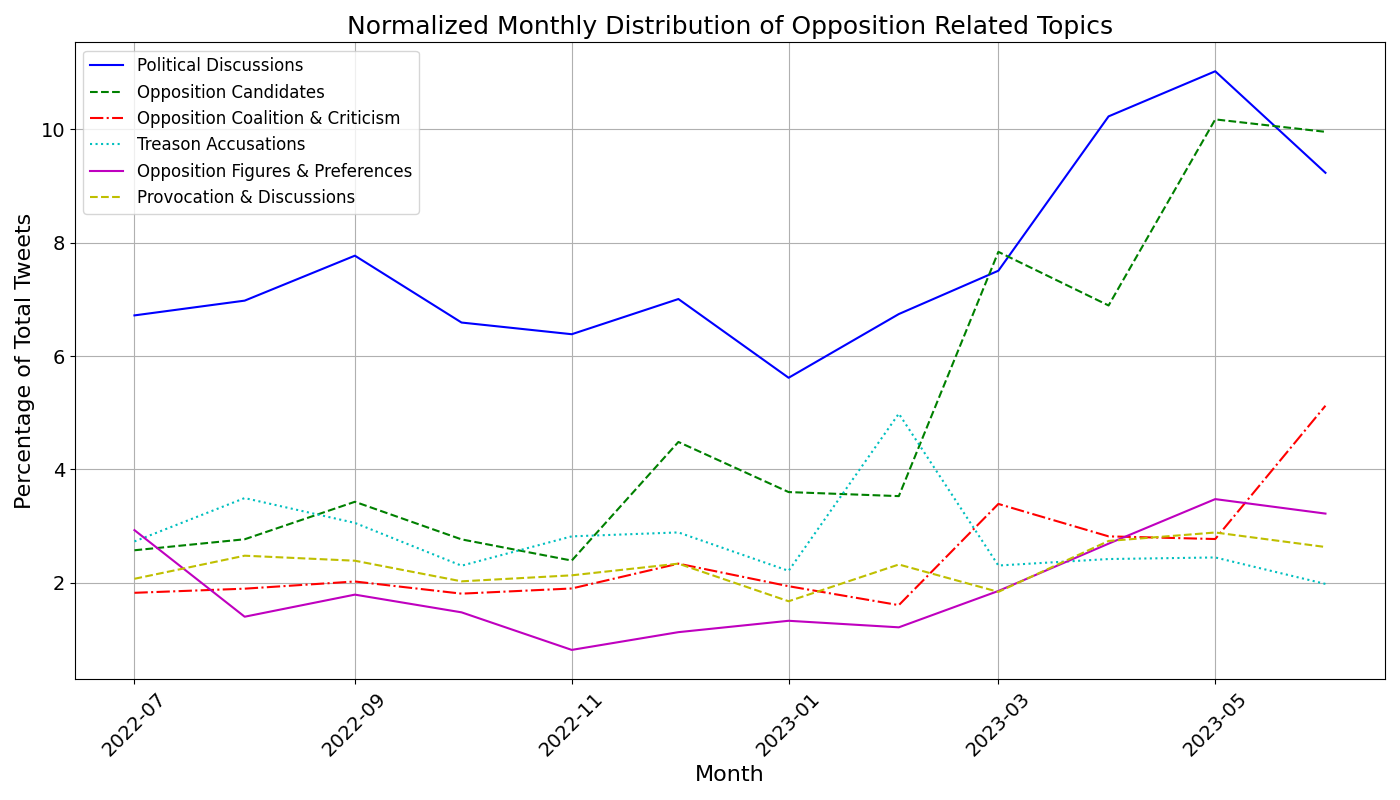
\includegraphics[width=\linewidth]{figures/normalized_opposition_selected_topics_distribution_with_styles.png}
    \caption[Normalized monthly distribution of opposition related topics]
    {Percentage of opposition related topics in the top 50 topics. 
    The blue line represents the biggest cluster and is the baseline, 
    and the other lines represent topics related to opposition parties and their candidates.}\label{fig:topics_graph_opposition}
\end{figure}

\begin{figure}[htb]
    \centering
    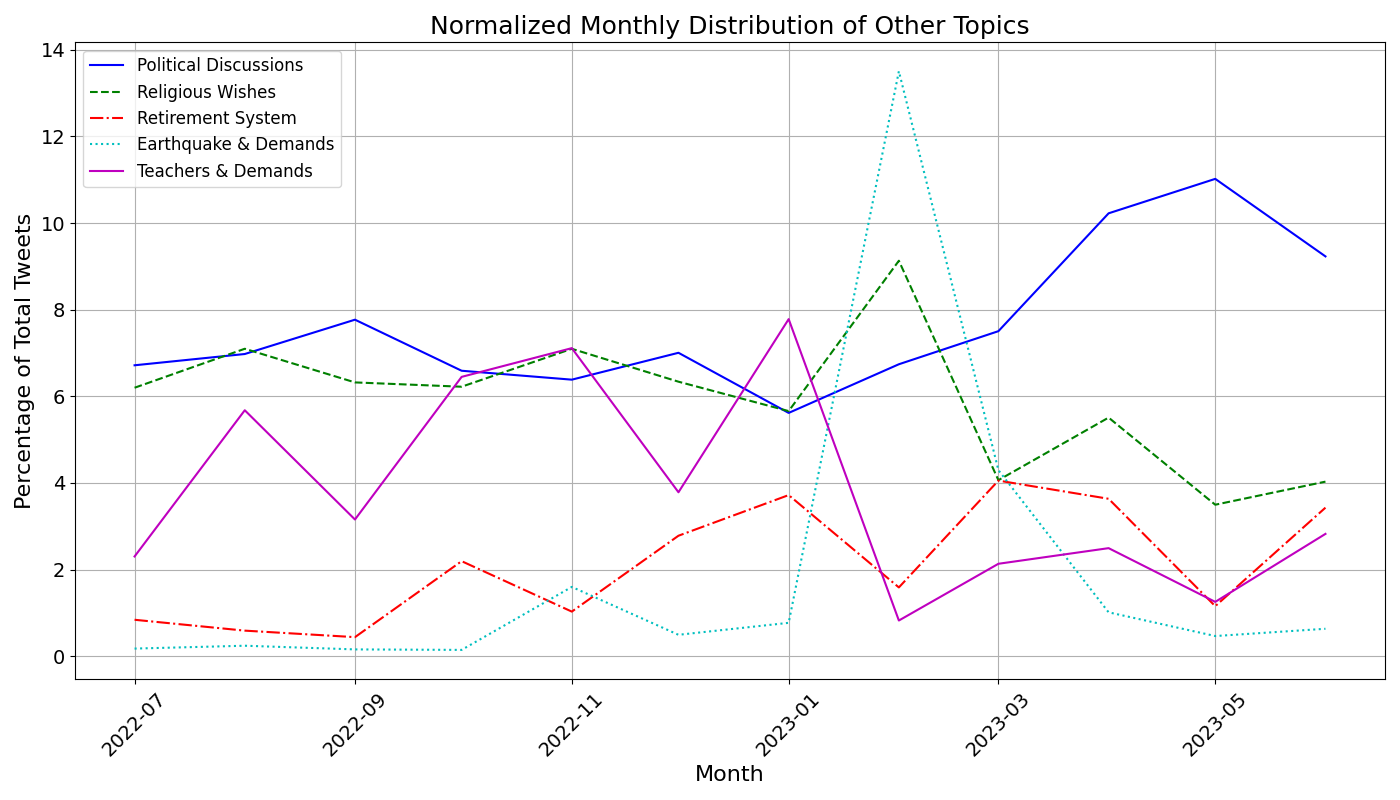
\includegraphics[width=\linewidth]{figures/normalized_other_selected_topics_distribution_with_styles.png}
    \caption[Normalized monthly distribution of other related topics]
    {Percentage of other related topics in the top 50 topics. 
    The blue line represents the biggest cluster and is the baseline, 
    and the other lines represent topics like demands from the government and the earthquake.}\label{fig:topics_graph_other}
\end{figure}



%  mention that topic is changed by me, ordered by frequency of it, after the transformation 
%  their order has cahnged. E.g. 7th topic was normally 24th before the transformation. 

% hierarchical topic model figure fig_hieararchy_50.html: 
% the top part represents requests from the government
% and the bottom part represents other topics

% percentage-wise graphs: show both of them, 
% in the second analysis because that there are less clusters
% the distribution makes it harder to see the trends and frequency 
% differences between topics


% add table of topics, keywords, openai labels
% add english/turkish one at the end of the thesis

% BELOW ARE TABLES COMMENTED OUT

% \begin{table}[htpb]
%     \centering
%     \begin{tabular}{|c c c|} 
%      \hline
%      \textbf{Topic} & \textbf{Count} & \textbf{Label} \\ [0.5ex] 
%      \hline\hline
%      1 & 4711805 & Elections, Candidates, and Political Discussions \\
%      2 & 2781739 & Erdogan and Political Developments \\
%      3 & 2704097 & Political Agenda and Demands \\
%      4 & 1561746 & Religious Wishes and Political Figures \\
%      5 & 1302418 & Teacher Appointments and Their Demands \\
%      6 & 1286107 & Earthquake and Relevant Requests \\
%      7 & 1222694 & Nation and Country \\
%      8 & 1049210 & Leading Figures in Turkish Politics \\
%      9 & 1022569 & Fair Trial and General Amnesty Requests \\
%      10 & 939330 & Mixed Emotions \\
%      11 & 873148 & Civil Servants and Their Demands \\
%      12 & 833265 & Retirement System and 5000 Premium Partial Retirement \\
%      13 & 813741 & Main Appointment Requests from Reserves \\
%      14 & 766576 & Medical Secretary Appointment Demands \\
%      15 & 759860 & 2023 Turkey Election News and Comments \\
%      16 & 704353 & Internship Grievances and Solution Calls \\
%      17 & 699035 & Staff Sergeant Position Demands \\
%      18 & 667885 & Industrial Internship Victims and Their Rights \\
%      19 & 640073 & Police Training Candidates Interview and Quota Requests \\
%      20 & 627449 & Political Dialogue in Hopes and Expectations \\
%      \hline
%     \end{tabular}
%     \caption[Result of the topic modeling]{Top 20 topics from the result of the topic modeling
%     with their respective topic label and count.}\label{tab:topic_modeling_results}
% \end{table}

% \begin{table}[htpb]
%     \centering
%     \begin{tabular}{|c | c | c|} 
%      \hline
%      \textbf{Topic} & \textbf{Count} & \textbf{Label} \\ [0.5ex] 
%      \hline\hline
%      1 & 4711805 & Seçimler, Adaylar ve Siyasi Tartışmalar \\
%      2 & 2781739 & Erdogan ve Türkiye Siyasi Gelişmeleri \\
%      3 & 2704097 & Türkiye Siyasi Gündem ve Talepler \\
%      4 & 1561746 & Dini Temenniler ve Siyasi Figürler \\
%      5 & 1302418 & Öğretmen Atamaları ve Talepleri \\
%      6 & 1286107 & Deprem Sonrası Yapı Kayıt Talebi \\
%      7 & 1222694 & Ülke ve Millet Konulu Siyasi Tartışma \\
%      8 & 1049210 & Türk Siyasetinde Önde Gelen Figürler \\
%      9 & 1022569 & Adil Yargılama ve Genel Af Talebi \\
%      10 & 939330 & Karışık Duygular ve İletişim Çıkmazı \\
%      11 & 873148 & Kamu Şefleri ve 3600 Ek Gösterge Talebi \\
%      12 & 833265 & EYT ve 5000 Prim Kısmi Emeklilik \\
%      13 & 813741 & Yedeklerin Asıl Atama Talebi \\
%      14 & 766576 & Tıbbi Sekreterlik Atama Talepleri \\
%      15 & 759860 & 2023 Türkiye Seçim Haberleri ve Yorumları \\
%      16 & 704353 & Staj Mağduriyeti ve Çözüm Çağrıları \\
%      17 & 699035 & Uzman Çavuşlar Kadro Talebi \\
%      18 & 667885 & Sanayide Staj Mağdurları ve Hakları \\
%      19 & 640073 & POMEM Adaylarının Mülakat ve Kontenjan Talebi \\
%      20 & 627449 & Umut ve Beklentilerde Siyasi Diyalog \\
%      \hline
%     \end{tabular}
%     \caption[Result of the topic modeling]{Top 20 topics from the result of the topic modeling
%     with their respective topic label and count.}\label{tab:topic_modeling_results3}
% \end{table}

% \begin{table}[htpb]
%     \resizebox{\textwidth}{!}{%
%     \centering
%     \begin{tabular}{|c|c|p{3cm}|p{7.5cm}|} 
%      \hline
%      \textbf{Topic} & \textbf{Count} & \textbf{Label} & \textbf{Representative words} \\ [0.5ex] 
%      \hline\hline
%      1 & 4711805 & Seçimler, Adaylar ve Siyasi Tartışmalar & oy, kılıçdaroğlu, aday, seçim, erdoğan, tayyip, seçimi, istifa, na, turda \\
%      2 & 2781739 & Erdogan ve Türkiye Siyasi Gelişmeleri & türk, türkiye, stanbul, yüzyılı, turkey, türkiyeyüzyılı, ankara, cumhuriyeti, erdogan, milleti \\
%      3 & 2704097 & Türkiye Siyasi Gündem ve Talepler & yirmiucderece, numankurtulmus, aysedogan1955, cenginyurt52, herkesicinchp, meral\_aksener, secimtr2023, hassa61, yildirimkaya40, yilmaztunc \\
%      4 & 1561746 & Dini Temenniler ve Siyasi Figürler & allah, versin, razı, eylesin, müslüman, etsin, din, rabbim, rahmet, cennet \\
%      5 & 1302418 & Öğretmen Atamaları ve Talepleri & öğretmen, öğretmenler, tcmeb, ataması, prof\_mahmutozer, 100, bin, kpss, öğretmenlerin, atama \\
%      6 & 1286107 & Deprem Sonrası Yapı Kayıt Talebi & deprem, depremde, depremzede, depremin, yapıkayıt, yumuşak, depremden, müstakil, planlayanlar, depreme \\
%      7 & 1222694 & Ülke ve Millet Konulu Siyasi Tartışma & ülkeyi, ülke, ülkenin, ülkeye, ülkede, millet, milletin, milleti, millete, senin \\
%      8 & 1049210 & Türk Siyasetinde Önde Gelen Figürler & başkanım, başkan, cumhurbaşkanım, mansuryavas06, ekrem\_imamoglu, başbakan, cumhurbaşkanı, sayın, genel, tanjuozcanchp \\
%      9 & 1022569 & Adil Yargılama ve Genel Af Talebi & mahkum, af, adalet, genelaf, 77, adil, adli, mahkumlar, ihlali, cezalar \\
%      10 & 939330 & Karışık Duygular ve İletişim Çıkmazı & que, me, eu, não, no, dedem, aq, amk, pra, lo \\
%      11 & 873148 & Kamu Şefleri ve 3600 Ek Gösterge Talebi & sırtlayan, hafızası, kurumların, yükünü, kamunun, 3600ekgösterge, devletine, umudumuz, sizsiniz, milletine \\
%      12 & 833265 & EYT ve 5000 Prim Kısmi Emeklilik & emeklilik, emekli, kısmi, kademeli, prim, 5000, yaş, zorunlu, 99, eyt \\
%      13 & 813741 & Yedeklerin Asıl Atama Talebi & degildi, tercihimiz, dileğimiz, milletvekilim, etmektir, yedek, talebimiz, mehmetfatihser5, vatandaşa, ittifakı \\
%      14 & 766576 & Tıbbi Sekreterlik Atama Talepleri & drfahrettinkoca, sağlık, 2020, tıbbi, sağlıkçılar, sekreterlik, sağlıkçı, yönetimi, suayipbirinci, saglikbakanligi \\
%      15 & 759860 & 2023 Türkiye Seçim Haberleri ve Yorumları & secimtr2023, yirmiucderece, cumhuriyetgzt, vekilince, https, co, ozan\_blk07, furkancerkes, gazetesozcu, herkesicinchp \\
%      16 & 704353 & Staj Mağduriyeti ve Çözüm Çağrıları & mağdurlari, kisa, sayin, çözülmeli, deği, üzmeyi, mahzun, alalim, mkalayci42, sürede \\
%      17 & 699035 & Uzman Çavuşlar Kadro Talebi & kadro, alitilkici38, çavuşlar, uzman, haktır, sırauzmançavuşakadro, yilmaz\_ismet58, 3269torbayasaya, uzmançavuşlartorbayasaya, çavuşlara \\
%      18 & 667885 & Sanayide Staj Mağdurları ve Hakları & mağdurları, sayildi, bedenleri, staj, büyüdü, çalişan, mağdurlarının, alin, teri, mağduriyeti \\
%      19 & 640073 & POMEM Adaylarının Mülakat ve Kontenjan Talebi & pomem, yedek, adayları, aliyerlikaya, 3546, ylmz\_colak, dönem, ergunyolcu, 29, 29dönempomem5binekkontenjan \\
%      20 & 627449 & Umut ve Beklentilerde Siyasi Diyalog & düşürmeyeceğinizden, umutlarımıza, gölge, eminiz, mehmetfatihser5, mehmetersoy57, düşeni, üzerimize, fazlasıyla, habere \\
%      \hline
%     \end{tabular}}
%     \caption[Result of the topic modeling]{Result of the topic modeling. Top ten representative words 
%     for each of top 20 topics with their respective topic label in Turkish.}\label{tab:topic_modeling_results2}
% \end{table}

% \begin{table}
%     \centering
%     \caption{Top 20 topics from the result of the topic modeling with their respective topic label and count.}\label{tab:topic_modeling_results23}
%     \begin{tabular}{|>{\centering\hspace{0pt}}m{0.07\linewidth}>{\centering\hspace{0pt}}m{0.1\linewidth}>{\centering\arraybackslash\hspace{0pt}}m{0.75\linewidth}|} 
%     \hline
%     \textbf{Topic} & \textbf{Count} & \textbf{Label}                                                           \\ 
%     \hline\hline
%     1              & 4711805        & Elections, Candidates, and Political Discussions                         \\
%     2              & 2781739        & Erdogan and Political Developments                                       \\
%     3              & 2704097        & Political Agenda and Demands                                             \\
%     4              & 1561746        & Religious Wishes and Political Figures                                   \\
%     5              & 1302418        & Teacher Appointments and Their Demands                                   \\
%     6              & 1286107        & Earthquake and Relevant Requests                                         \\
%     7              & 1222694        & Nation and Country                                                       \\
%     8              & 1049210        & Leading Figures in Turkish Politics                                      \\
%     9              & 1022569        & Fair Trial and General Amnesty Requests                                  \\
%     10             & 939330         & Mixed Emotions                                                           \\
%     11             & 873148         & Public Officials and the 3600 Additional Indicator Demand                \\
%     12             & 833265         & EYT (Retirement Benefit System) and 5000 Premium Partial Retirement      \\
%     13             & 813741         & Main Appointment Requests from Reserves                                  \\
%     14             & 766576         & Medical Secretary Appointment Demands                                    \\
%     15             & 759860         & Election News and Comments                                               \\
%     16             & 704353         & Internship Grievances and Solution Calls                                 \\
%     17             & 699035         & Staff Sergeant Position Demands                                          \\
%     18             & 667885         & Industrial Internship Victims and Their Rights                           \\
%     19             & 640073         & POMEM (Police Training Center) Candidates Interview and Quota Requests  \\
%     20             & 627449         & Political Dialogue in Hopes and Expectations                             \\
%     \hline
%     \end{tabular}
%     \end{table}

% \begin{table}
% \centering
% \caption{Result of the topic modeling. Top ten representative words for each of top 20 topics with their respective topic label in Turkish.}
% \label{tab:topic_modeling_results23}
% \begin{tabular}{|>{\centering\hspace{0pt}}m{0.05\linewidth}|>{\centering\hspace{0pt}}m{0.06\linewidth}|>{\hspace{0pt}}m{0.221\linewidth}|>{\hspace{0pt}}m{0.608\linewidth}|} 
% \hline
% \textbf{Topic} & \textbf{Count} & \textbf{Label}                                & \textbf{Representative words}                                                                                                                \\ 
% \hline\hline
% 1             & 4711805        & Seçimler, Adaylar ve Siyasi Tartışmalar       & oy, kılıçdaroğlu, aday, seçim, erdoğan, tayyip, seçimi, istifa, na, turda                                                                    \\
% 2              & 2781739        & Erdogan ve Türkiye Siyasi Gelişmeleri         & türk, türkiye, stanbul, yüzyılı, turkey, türkiyeyüzyılı, ankara, cumhuriyeti, erdogan, milleti                                               \\
% 3              & 2704097        & Türkiye Siyasi Gündem ve Talepler             & yirmiucderece, numankurtulmus, aysedogan1955, cenginyurt52, herkesicinchp, meral\_aksener, secimtr2023, hassa61, yildirimkaya40, yilmaztunc  \\
% 4              & 1561746        & Dini Temenniler ve Siyasi Figürler            & allah, versin, razı, eylesin, müslüman, etsin, din, rabbim, rahmet, cennet                                                                   \\
% 5              & 1302418        & Öğretmen Atamaları ve Talepleri               & öğretmen, öğretmenler, tcmeb, ataması, prof\_mahmutozer, 100, bin, kpss, öğretmenlerin, atama                                                \\
% 6              & 1286107        & Deprem Sonrası Yapı Kayıt Talebi              & deprem, depremde, depremzede, depremin, yapıkayıt, yumuşak, depremden, müstakil, planlayanlar, depreme                                       \\
% 7              & 1222694        & Ülke ve Millet Konulu Siyasi Tartışma         & ülkeyi, ülke, ülkenin, ülkeye, ülkede, millet, milletin, milleti, millete, senin                                                             \\
% 8              & 1049210        & Türk Siyasetinde Önde Gelen Figürler          & başkanım, başkan, cumhurbaşkanım, mansuryavas06, ekrem\_imamoglu, başbakan, cumhurbaşkanı, sayın, genel, tanjuozcanchp                       \\
% 9              & 1022569        & Adil Yargılama ve Genel Af Talebi             & mahkum, af, adalet, genelaf, 77, adil, adli, mahkumlar, ihlali, cezalar                                                                      \\
% 10             & 939330         & Karışık Duygular ve İletişim Çıkmazı          & que, me, eu, não, no, dedem, aq, amk, pra, lo                                                                                                \\
% 11             & 873148         & Kamu Şefleri ve 3600 Ek Gösterge Talebi       & sırtlayan, hafızası, kurumların, yükünü, kamunun, 3600ekgösterge, devletine, umudumuz, sizsiniz, milletine                                   \\
% 12             & 833265         & EYT ve 5000 Prim Kısmi Emeklilik              & emeklilik, emekli, kısmi, kademeli, prim, 5000, yaş, zorunlu, 99, eyt                                                                        \\
% 13             & 813741         & Yedeklerin Asıl Atama Talebi                  & degildi, tercihimiz, dileğimiz, milletvekilim, etmektir, yedek, talebimiz, mehmetfatihser5, vatandaşa, ittifakı                              \\
% 14             & 766576         & Tıbbi Sekreterlik Atama Talepleri             & drfahrettinkoca, sağlık, 2020, tıbbi, sağlıkçılar, sekreterlik, sağlıkçı, yönetimi, suayipbirinci, saglikbakanligi                           \\
% 15             & 759860         & 2023 Türkiye Seçim Haberleri ve Yorumları     & secimtr2023, yirmiucderece, cumhuriyetgzt, vekilince, https, co, ozan\_blk07, furkancerkes, gazetesozcu, herkesicinchp                       \\
% \hline
% \end{tabular}
% \end{table}

% \begin{table}
%     \centering
%     \begin{tabular}{|>{\centering\hspace{0pt}}m{0.052\linewidth}|>{\hspace{0pt}}m{0.223\linewidth}|>{\hspace{0pt}}m{0.665\linewidth}|} 
%     \hline
%     \textbf{Topic} & \textbf{Label}                                 & \textbf{Representative words}                                                                                                                \\ 
%     \hline\hline
%     1             & Elections and Candidates                       & oy, kılıçdaroğlu, aday, seçim, erdoğan, tayyip, seçimi, istifa, na, turda                                                                    \\
%     2              & Erdogan and Political Developments             & türk, türkiye, stanbul, yüzyılı, turkey, türkiyeyüzyılı, ankara, cumhuriyeti, erdogan, milleti                                               \\
%     3              & Political Agenda and Demands                   & yirmiucderece, numankurtulmus, aysedogan1955, cenginyurt52, herkesicinchp, meral\_aksener, secimtr2023, hassa61, yildirimkaya40, yilmaztunc  \\
%     4              & Religious Wishes and Political Figures         & allah, versin, razı, eylesin, müslüman, etsin, din, rabbim, rahmet, cennet                                                                   \\
%     5              & Teacher Appointments and Their Demands         & öğretmen, öğretmenler, tcmeb, ataması, prof\_mahmutozer, 100, bin, kpss, öğretmenlerin, atama                                                \\
%     6              & Earthquake and Relevant Demands                & deprem, depremde, depremzede, depremin, yapıkayıt, yumuşak, depremden, müstakil, planlayanlar, depreme                                       \\
%     7              & Nation and Country                             & ülkeyi, ülke, ülkenin, ülkeye, ülkede, millet, milletin, milleti, millete, senin                                                             \\
%     8              & Leading Figures                                & başkanım, başkan, cumhurbaşkanım, mansuryavas06, ekrem\_imamoglu, başbakan, cumhurbaşkanı, sayın, genel, tanjuozcanchp                       \\
%     9              & Fair Trial and General Amnesty Requests        & mahkum, af, adalet, genelaf, 77, adil, adli, mahkumlar, ihlali, cezalar                                                                      \\
%     10             & Mixed Emotions                                 & que, me, eu, não, no, dedem, aq, amk, pra, lo                                                                                                \\
%     11             & Civil Servants and Their Demands               & sırtlayan, hafızası, kurumların, yükünü, kamunun, 3600ekgösterge, devletine, umudumuz, sizsiniz, milletine                                   \\
%     12             & Retirement System                              & emeklilik, emekli, kısmi, kademeli, prim, 5000, yaş, zorunlu, 99, eyt                                                                        \\
%     13             & Appointment Demands from Reserves              & degildi, tercihimiz, dileğimiz, milletvekilim, etmektir, yedek, talebimiz, mehmetfatihser5, vatandaşa, ittifakı                              \\
%     14             & Medical Secretary Appointment Demands          & drfahrettinkoca, sağlık, 2020, tıbbi, sağlıkçılar, sekreterlik, sağlıkçı, yönetimi, suayipbirinci, saglikbakanligi                           \\
%     15             & Election News and Comments                     & secimtr2023, yirmiucderece, cumhuriyetgzt, vekilince, https, co, ozan\_blk07, furkancerkes, gazetesozcu, herkesicinchp                       \\
%     16             & Internship Grievances and Solution Calls       & mağdurlari, kisa, sayin, çözülmeli, deği, üzmeyi, mahzun, alalim, mkalayci42, sürede                                                         \\
%     17             & Staff Sergeant Position Demands                & kadro, alitilkici38, çavuşlar, uzman, haktır, sırauzmançavuşakadro, yilmaz\_ismet58, 3269torbayasaya, uzmançavuşlartorbayasaya, çavuşlara    \\
%     18             & Industrial Internship Victims and Their Rights & mağdurları, sayildi, bedenleri, staj, büyüdü, çalişan, mağdurlarının, alin, teri, mağduriyeti                                                \\
%     19             & Police Training Candidates Demands            & pomem, yedek, adayları, aliyerlikaya, 3546, ylmz\_colak, dönem, ergunyolcu, 29, 29dönempomem5binekkontenjan                                  \\
%     20             & Political Dialogue in Hopes and Expectations   & düşürmeyeceğinizden, umutlarımıza, gölge, eminiz, mehmetfatihser5, mehmetersoy57, düşeni, üzerimize, fazlasıyla, habere                      \\
%     \hline
%     \end{tabular}
%     \caption{Result of the topic modeling. Top ten representative words
%     for each of top 20 topics with their respective topic label in Turkish.}\label{tab:topic_modeling_results232}
%     \end{table}
